% !TeX root = ../main.tex
\chapter[Unidad 8: Enfermedades y estudios auditivos, técnicas de rehabilitación]{Unidad 8: Alteraciones y enfermedades auditivas, estudios y técnicas de rehabilitación}
\label{chap:unidad-8}

\section{Propósito y resultados de aprendizaje}
\label{sec:u8-proposito}

Una dificultad para comprender el habla, un cambio en el umbral auditivo y
la percepción de un acúfeno no describen el mismo fenómeno. La primera es
una limitación comunicativa; el segundo es un resultado conductual expresado
en una escala audiométrica; la tercera es una experiencia perceptual. Pueden
coexistir, pero no deben confundirse ni atribuirse automáticamente a una
misma causa.

Esta unidad propone un marco físico para relacionar tres conjuntos de
contenidos: alteraciones y enfermedades auditivas, estudios y dispositivos de
rehabilitación. No constituye una guía para diagnosticar ni indicar
tratamientos. El diagnóstico clínico y la selección de una intervención
requieren integrar antecedentes, examen profesional y resultados obtenidos
con procedimientos validados.

Al finalizar la unidad se espera que podamos:

\begin{itemize}
    \item diferenciar una exposición física, una alteración de la función
    auditiva, un resultado de medición y un atributo perceptual;
    \item explicar, con alcance introductorio, el desplazamiento temporal
    del umbral, la pérdida auditiva inducida por ruido, el trauma acústico,
    el tinnitus, la presbiacusia y la ototoxicidad;
    \item describir para cada estudio el estímulo, la magnitud registrada,
    la parte del sistema auditivo explorada, la participación conductual, el
    resultado básico y sus limitaciones generales;
    \item interpretar ejemplos conceptuales de audiometría tonal,
    logoaudiometría, timpanometría, acufenometría, otoemisiones acústicas,
    potenciales auditivos evocados y electrococleografía sin convertir un
    patrón aislado en un diagnóstico;
    \item comparar las transformaciones físicas realizadas por un audífono,
    un implante coclear y un dispositivo de conducción ósea;
    \item resolver cálculos sencillos de exposición equivalente, diferencia
    entre vías audiométricas y ganancia electroacústica, declarando las
    hipótesis y las unidades.
\end{itemize}

\section{Conocimientos previos}
\label{sec:u8-previos}

Conviene recuperar cuatro distinciones desarrolladas anteriormente:

\begin{itemize}
    \item los niveles en decibeles son relaciones logarítmicas y cada
    descriptor debe incluir su referencia o ponderación
    (Sección~\ref{sec:u4-niveles-auditivos});
    \item un espectro describe el contenido frecuencial de una señal, mientras
    que una respuesta en frecuencia caracteriza a un sistema
    (Unidad~\ref{chap:unidad-5});
    \item las vías aérea y ósea involucran mecanismos físicos diferentes
    (Unidad~\ref{chap:unidad-6});
    \item frecuencia, altura tonal, presión sonora, sonoridad y nivel de
    audición no son términos intercambiables
    (Unidad~\ref{chap:unidad-7}).
\end{itemize}

La Unidad~\ref{chap:unidad-6} presentó el funcionamiento auditivo habitual y
la Unidad~\ref{chap:unidad-7} estudió relaciones psicofísicas. Aquí esos
conceptos se aplican a
alteraciones, pruebas y dispositivos. La caracterización de fuentes de ruido
y el enmascaramiento ambiental se retoman con mayor detalle en la
Unidad~\ref{chap:unidad-10}.

\section{Situación introductoria: una queja, varias preguntas}
\label{sec:u8-situacion}

Una persona refiere que, después de trabajar, necesita aumentar el nivel del
televisor, le cuesta seguir conversaciones en ambientes ruidosos y percibe un
sonido sin identificar una fuente externa. Antes de proponer una explicación,
es necesario separar preguntas distintas:

\begin{enumerate}
    \item ¿cómo fue la exposición acústica: nivel, duración, espectro e
    impulsividad?;
    \item ¿cambió el umbral conductual y, si cambió, en qué frecuencias?;
    \item ¿cómo se comporta la transferencia del oído medio?;
    \item ¿se registra una respuesta coclear o neural ante un estímulo
    controlado?;
    \item ¿qué limitación comunicativa describe la persona?;
    \item ¿qué dispositivo podría transformar la señal de una manera útil,
    una vez realizada la evaluación correspondiente?
\end{enumerate}

Ninguna de estas preguntas reemplaza a las demás. Ésta es la idea organizadora
del capítulo.

\section{Bloque I. Alteraciones y patologías}
\label{sec:u8-alteraciones}

\subsection{Exposición, lesión, síntoma y resultado}

El nivel de presión sonora, el espectro y la duración caracterizan una
\emph{exposición}. Un cambio en estructuras o funciones auditivas es una
\emph{alteración}. El tinnitus o la dificultad para comprender el habla son
\emph{experiencias o síntomas}. Un umbral en dB HL es un \emph{resultado de
medición}. Estas categorías pueden relacionarse, pero una no demuestra por sí
sola la presencia de las otras.

En la práctica audiológica se suele distinguir entre componentes
conductivos, sensorioneurales y mixtos según las partes del sistema auditivo
comprometidas; esta clasificación debe integrarse con la historia clínica y
con una batería de pruebas, no inferirse de un único dato~\cite{ashaHearingAdults}.

\subsection{Desplazamiento temporal del umbral y exposición a ruido}
\label{sec:u8-tts}

El \textbf{desplazamiento temporal del umbral} (\emph{temporary threshold
shift}, TTS) describe una diferencia entre dos mediciones de umbral separadas
en el tiempo. No describe un zumbido ni el nivel físico del sonido que produjo
la exposición.

Sea \(f\) la frecuencia del tono de prueba, expresada en hertz
(\(\mathrm{Hz}\)); sea \(L_{\mathrm{U},0}(f)\) el nivel de audición del umbral
de referencia, expresado en decibeles de nivel de audición
(\(\mathrm{dB\,HL}\)); y sea \(L_{\mathrm{U},1}(f,\Delta t)\) el umbral medido
un intervalo \(\Delta t\) después de la exposición, también en
\(\mathrm{dB\,HL}\). Se define:

\begin{equation}
    \Delta L_{\mathrm{T}}(f,\Delta t)
    =
    L_{\mathrm{U},1}(f,\Delta t)-L_{\mathrm{U},0}(f),
    \label{eq:u8-tts}
\end{equation}

donde \(\Delta L_{\mathrm{T}}\) se expresa en decibeles (\(\mathrm{dB}\)).
Un valor positivo indica que, en esa medición, fue necesario un nivel de
audición mayor para obtener la respuesta. La ecuación no identifica por sí
misma el mecanismo biológico ni establece si la diferencia es clínicamente
significativa.

La magnitud y el curso temporal de un TTS dependen, entre otros
factores, del nivel, el espectro y la duración de la exposición, del tiempo
transcurrido hasta la medición y de la variabilidad individual. Las
afirmaciones sobre tiempos de recuperación o mecanismos celulares requieren
una fuente primaria y no deben expresarse como intervalos universales~\cite{ryan2016}.

La \textbf{pérdida auditiva inducida por ruido} (PAIR; también denominada
NIHL por su sigla en inglés) se refiere a cambios auditivos permanentes
asociados con exposición a ruido. Su evaluación requiere integrar la
historia de exposición, el patrón audiométrico y otras causas posibles. Una
escotadura en el audiograma puede ser compatible con exposición a ruido, pero
no demuestra por sí sola su etiología~\cite{ryan2016,ashaHearingAdults}.

Desde la física, el riesgo no puede resumirse en ``muchos decibeles''. Deben
declararse el descriptor de nivel, la ponderación frecuencial, el intervalo
temporal, el espectro y la presencia de impulsos o picos. Los conceptos de
nivel equivalente se desarrollaron en la Sección~\ref{sec:u5-leq}.

\medskip
\noindent\textbf{Ejemplo físico: normalización temporal.}\par
Supongamos, sólo con fines didácticos, que una fuente produce durante una hora
un nivel sonoro continuo equivalente ponderado A
\(L_{A\mathrm{eq},1\,\mathrm{h}}=95\,\mathrm{dB(A)}\) y que su contribución durante las
otras siete horas es despreciable. Para expresar la misma energía sonora
promedio en un intervalo de ocho horas:

\begin{equation}
    L_{A\mathrm{eq},8\,\mathrm{h}}
    =
    L_{A\mathrm{eq},1\,\mathrm{h}}
    +10\log_{10}\left(\frac{1\,\mathrm{h}}{8\,\mathrm{h}}\right)
    \simeq 86{,}0\,\mathrm{dB(A)}.
    \label{eq:u8-leq-ejemplo}
\end{equation}

El cociente entre tiempos es adimensional. Este resultado compara energías
promedio bajo las hipótesis indicadas; no establece por sí solo que la
exposición sea segura, legal o aceptable. La evaluación ocupacional
debe aplicar la normativa vigente en la jurisdicción correspondiente,
incluidos sus criterios para ruido continuo, variable e impulsivo y para el
uso de protección auditiva~\cite{argentinaResolucion85,nioshNoise1998}.

\subsection{Trauma acústico y ototoxicidad}
\label{sec:u8-trauma}

El \textbf{trauma acústico} se asocia con un episodio acústico abrupto
y de alta energía, por ejemplo una explosión~\cite{ryan2016,kurabi2017}. Según las características
del evento, puede comprometer estructuras del oído externo, medio o interno;
el nivel de pico aislado no permite predecir de manera universal la lesión~\cite{ryan2016,kurabi2017}.
Por eso deben registrarse, cuando sea posible, la forma temporal, el espectro,
la duración y el contexto del evento, además de los síntomas referidos.

Este capítulo no indica conductas terapéuticas. La aparición súbita de
síntomas auditivos o vestibulares después de un evento intenso requiere
evaluación sanitaria oportuna de acuerdo con protocolos clínicos vigentes~\cite{ashaHearingAdults}.

La \textbf{ototoxicidad} no es una propiedad acústica de un sonido.
Ciertos medicamentos y agentes químicos pueden afectar funciones
cocleares o vestibulares. El riesgo depende del agente, la dosis acumulada,
la vía de administración, factores individuales y exposiciones concurrentes~\cite{nioshOtotoxic2018}.
El aporte de la medición consiste en comparar registros seriados obtenidos con
procedimientos controlados; cualquier decisión farmacológica corresponde al
equipo tratante.

\subsection{Tinnitus o acúfeno}
\label{sec:u8-tinnitus}

El \textbf{tinnitus} o \textbf{acúfeno} es una percepción sonora
referida sin que exista una fuente acústica externa correspondiente~\cite{ashaTinnitus}.
La mayoría de
los casos se describe como tinnitus subjetivo; existen situaciones menos
frecuentes en las que un sonido generado dentro del organismo puede ser
detectable por un observador~\cite{ashaTinnitus}.

La persona puede comparar su percepción con tonos o ruidos presentados por un
equipo. La frecuencia del tono elegido se expresa en \(\mathrm{Hz}\), pero
representa una \emph{correspondencia perceptual} y no una medición directa de
una oscilación física dentro del oído. Del mismo modo, un nivel de
comparación expresado en \(\mathrm{dB\,SL}\) no es la ``intensidad física del
tinnitus''. La acufenometría se estudia en la
Sección~\ref{sec:u8-acufenometria}.

El tinnitus puede coexistir con umbrales audiométricos diversos y con
condiciones auditivas o no auditivas diferentes. Su evaluación clínica no
debe reducirse a una única correspondencia de frecuencia o nivel~\cite{ashaTinnitus}.

\subsection{Presbiacusia}
\label{sec:u8-presbiacusia}

La \textbf{presbiacusia} designa cambios auditivos asociados con el
envejecimiento~\cite{gatesMills2005}. Es un proceso heterogéneo y multifactorial en el que
pueden intervenir cambios cocleares, neurales y metabólicos, además de la
historia de exposición a ruido, enfermedades y medicamentos. Suele
describirse como bilateral y con mayor compromiso de frecuencias altas, pero
no existe una pendiente audiométrica única que defina todos los casos~\cite{gatesMills2005}.

Un audiograma descendente muestra umbrales mayores en frecuencias altas; es
una descripción geométrica del registro, no una etiología. La edad tampoco
convierte automáticamente ese patrón en presbiacusia.

\section{Bloque II. Estudios diagnósticos}
\label{sec:u8-estudios}

\subsection{Una cadena común para comparar pruebas}
\label{sec:u8-cadena-medicion}

Todo estudio puede analizarse como una cadena. Un estímulo controlado actúa
sobre el sistema auditivo; la respuesta resultante llega a un sensor o a una
tarea conductual; y el dato registrado se interpreta dentro de los límites
del procedimiento.

Las pruebas \textbf{conductuales} requieren una acción de la persona,
por ejemplo presionar un pulsador o repetir una palabra. Las pruebas
\textbf{fisiológicas} registran una señal acústica, mecánica o bioeléctrica y
no requieren esa respuesta voluntaria, aunque sí exigen condiciones de
registro adecuadas~\cite{ashaHearingAdults}. ``Objetiva'' no significa automática, infalible ni
independiente de la preparación y del análisis profesional.

\begin{table}[htbp]
    \centering
    \caption{Relación introductoria entre la función explorada y las pruebas.
    Una prueba puede depender de más de una parte del sistema y ninguna fila
    equivale por sí sola a un diagnóstico.}
    \label{tab:u8-estructura-prueba}
    \small
    \setlength{\tabcolsep}{3pt}
    \begin{tabular}{
        >{\raggedright\arraybackslash}p{0.24\textwidth}
        >{\raggedright\arraybackslash}p{0.29\textwidth}
        >{\raggedright\arraybackslash}p{0.37\textwidth}}
        \hline
        \textbf{Estructura o función} &
        \textbf{Pruebas relacionadas} &
        \textbf{Precaución interpretativa} \\
        \hline
        Transferencia por oído externo y medio &
        Audiometría por vía aérea, timpanometría, OEA &
        Una alteración de la transmisión puede modificar pruebas dirigidas
        principalmente a otras estructuras. \\
        Función coclear &
        Audiometría tonal, OEA, electrococleografía &
        Una respuesta presente no describe por sí sola toda la audición. \\
        Nervio auditivo y tronco encefálico &
        Potenciales auditivos evocados, electrococleografía &
        El registro neural no equivale a comprensión del habla. \\
        Respuesta auditiva integrada y percepción &
        Audiometría tonal, logoaudiometría, acufenometría &
        Depende de la consigna, la atención y las características del
        material. \\
        \hline
    \end{tabular}
\end{table}

\subsection{Audiometría tonal liminar}
\label{sec:u8-audiometria}

\begin{description}[style=nextline]
    \item[Estímulo.]
    Tonos de frecuencia y nivel controlados, presentados por vía aérea
    mediante auriculares o por vía ósea mediante un vibrador~\cite{ashaHearingAdults,ashaPureTone2005,iso8253_1_2010}.

    \item[Magnitud registrada.]
    Nivel de audición del umbral para cada frecuencia, expresado en
    \(\mathrm{dB\,HL}\). El eje horizontal del audiograma representa
    frecuencia en \(\mathrm{Hz}\); el vertical, nivel de audición en
    \(\mathrm{dB\,HL}\)~\cite{ashaHearingAdults,ashaPureTone2005,iso8253_1_2010}.

    \item[Parte del sistema evaluada.]
    La vía aérea depende de la cadena completa desde el oído externo hasta la
    respuesta conductual. La vía ósea modifica la forma de estimular las
    cócleas, pero no constituye una medición aislada de una única estructura~\cite{ashaHearingAdults,ashaPureTone2005,iso8253_1_2010}.

    \item[Respuesta conductual.]
    Sí. La persona indica la detección del estímulo según una consigna
    y un procedimiento de búsqueda de umbral~\cite{ashaHearingAdults,ashaPureTone2005,iso8253_1_2010}.

    \item[Resultado básico esperado.]
    Un audiograma con umbrales por frecuencia, oído y vía. La
    simbología, las frecuencias examinadas y el procedimiento de
    enmascaramiento deben seguir normas audiométricas vigentes~\cite{ashaHearingAdults,ashaPureTone2005,iso8253_1_2010}.

    \item[Limitaciones generales.]
    Influyen la calibración, el ruido ambiente, la colocación del transductor,
    la comprensión de la consigna, la fiabilidad de la respuesta y el
    enmascaramiento entre oídos. Un patrón no determina por sí solo una
    etiología~\cite{ashaHearingAdults,ashaPureTone2005,iso8253_1_2010}.
\end{description}

Sea \(L_{\mathrm{VA}}(f)\) el umbral por vía aérea y
\(L_{\mathrm{VO}}(f)\) el umbral por vía ósea, ambos en
\(\mathrm{dB\,HL}\), para la frecuencia \(f\) en \(\mathrm{Hz}\). La
diferencia entre vías puede escribirse:

\begin{equation}
    G_{\mathrm{AO}}(f)
    =
    L_{\mathrm{VA}}(f)-L_{\mathrm{VO}}(f),
    \label{eq:u8-gap}
\end{equation}

donde \(G_{\mathrm{AO}}\) se expresa en \(\mathrm{dB}\). Por ejemplo, con
datos didácticos ficticios, si a \(1000\,\mathrm{Hz}\) se registran
\(L_{\mathrm{VA}}=40\,\mathrm{dB\,HL}\) y
\(L_{\mathrm{VO}}=15\,\mathrm{dB\,HL}\), entonces
\(G_{\mathrm{AO}}=25\,\mathrm{dB}\). La resta describe la diferencia
obtenida en esas condiciones; no autoriza a nombrar una enfermedad.

La figura~\ref{fig:u8-audiograma-conceptual} aplica estas convenciones a un
registro ficticio. Su propósito es enseñar a leer los ejes y a comparar vías,
no representar una patología.

\begin{figure}[htbp]
    \centering
    % Propósito: enseñar la convención de lectura de un audiograma y mostrar que
% la diferencia entre vía aérea y vía ósea se calcula frecuencia por frecuencia.
% Origen: definición de G_AO(f) en \eqref{eq:u8-gap}. Los seis pares de puntos
% son datos didácticos ficticios, no mediciones, normas ni patrones diagnósticos.
% Las frecuencias de octava se ubican a distancias iguales, equivalentes a un
% eje logarítmico de base 2. En 1000 Hz se reproducen los valores del ejemplo
% del texto: 40 dB HL por vía aérea y 15 dB HL por vía ósea.
% Descripción accesible: el eje horizontal muestra frecuencias entre 250 y
% 8000 Hz en posiciones de octava. El eje vertical muestra nivel de audición
% en dB HL y aumenta hacia abajo según la convención audiométrica. Dos trazos
% ficticios representan vía aérea y vía ósea. En 1000 Hz una flecha vertical
% marca una diferencia de 25 dB, sin atribuirle diagnóstico.
% Validación prevista: comprobar el sentido del eje vertical, las etiquetas y
% unidades, la separación entre rótulo y números del eje vertical, la posición
% de las frecuencias sobre el eje, la resta 40 dB HL - 15 dB HL = 25 dB y la
% legibilidad en página.
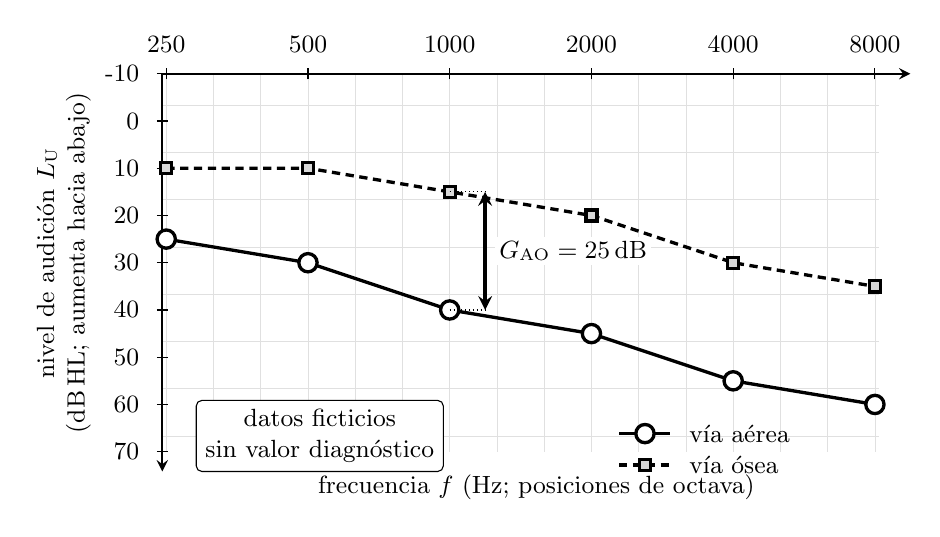
\begin{tikzpicture}[font=\small,>=stealth,x=1cm,y=1cm]
    \draw[step=0.60cm,black!12,very thin] (1.15,0.40) grid (10.25,5.20);

    \draw[->,thick] (1.15,5.20) -- (1.15,0.15);
    \draw[->,thick] (1.15,5.20) -- (10.65,5.20);
    \node[rotate=90,align=center] at (-0.10,2.80)
        {nivel de audición \(L_\mathrm{U}\)\\(\(\mathrm{dB\,HL}\); aumenta hacia abajo)};
    \node[align=center] at (5.90,-0.05)
        {frecuencia \(f\) (\(\mathrm{Hz}\); posiciones de octava)};

    \foreach \y/\lab in {
        5.20/-10,4.60/0,4.00/10,3.40/20,2.80/30,
        2.20/40,1.60/50,1.00/60,0.40/70}{
        \draw (1.08,\y) -- (1.22,\y);
        \node[anchor=east] at (0.98,\y) {\lab};
    }

    \foreach \x/\lab in {
        1.20/250,3.00/500,4.80/1000,6.60/2000,8.40/4000,10.20/8000}{
        \draw (\x,5.13) -- (\x,5.27);
        \node[anchor=south] at (\x,5.34) {\lab};
    }

    % Vía aérea ficticia: 25, 30, 40, 45, 55 y 60 dB HL.
    \draw[very thick]
        plot coordinates {
            (1.20,3.10) (3.00,2.80) (4.80,2.20)
            (6.60,1.90) (8.40,1.30) (10.20,1.00)
        };
    \foreach \x/\y in {
        1.20/3.10,3.00/2.80,4.80/2.20,
        6.60/1.90,8.40/1.30,10.20/1.00}{
        \draw[very thick,fill=white] (\x,\y) circle (3.3pt);
    }

    % Vía ósea ficticia: 10, 10, 15, 20, 30 y 35 dB HL.
    \draw[very thick,densely dashed]
        plot coordinates {
            (1.20,4.00) (3.00,4.00) (4.80,3.70)
            (6.60,3.40) (8.40,2.80) (10.20,2.50)
        };
    \foreach \x/\y in {
        1.20/4.00,3.00/4.00,4.80/3.70,
        6.60/3.40,8.40/2.80,10.20/2.50}{
        \draw[very thick,fill=black!15] (\x-0.07,\y-0.07) rectangle ++(0.14,0.14);
    }

    \draw[densely dotted] (4.80,2.20) -- (5.25,2.20);
    \draw[densely dotted] (4.80,3.70) -- (5.25,3.70);
    \draw[<->,very thick] (5.25,2.20) -- (5.25,3.70)
        node[midway,right=3pt,fill=white,inner sep=1.5pt]
        {\(G_{\mathrm{AO}}=25\,\mathrm{dB}\)};

    \draw[very thick] (6.95,0.63) -- (7.60,0.63);
    \draw[very thick,fill=white] (7.28,0.63) circle (3.3pt);
    \node[anchor=west] at (7.72,0.63) {vía aérea};
    \draw[very thick,densely dashed] (6.95,0.23) -- (7.60,0.23);
    \draw[very thick,fill=black!15] (7.21,0.16) rectangle ++(0.14,0.14);
    \node[anchor=west] at (7.72,0.23) {vía ósea};

    \node[draw,rounded corners=2pt,fill=white,align=center]
        at (3.15,0.60)
        {datos ficticios\\sin valor diagnóstico};
\end{tikzpicture}

    \caption{Audiograma conceptual con datos didácticos ficticios. Las
    frecuencias de octava se disponen horizontalmente y el nivel de audición
    en \(\mathrm{dB\,HL}\) aumenta hacia abajo según la convención
    audiométrica. La flecha muestra cómo se obtiene
    \(G_{\mathrm{AO}}=25\,\mathrm{dB}\) a \(1000\,\mathrm{Hz}\). Los trazos no
    proceden de una medición, no representan un patrón normativo y no poseen
    valor diagnóstico; elaboración propia.}
    \label{fig:u8-audiograma-conceptual}
    \label{fig:presbiacusia}
\end{figure}

\subsection{Logoaudiometría}
\label{sec:u8-logoaudiometria}

\begin{description}[style=nextline]
    \item[Estímulo.]
    Material verbal grabado o presentado de manera controlada, a
    niveles especificados por el procedimiento~\cite{ashaHearingAdults,ashaPureTone2005,iso8253_1_2010}.

    \item[Magnitud registrada.]
    Según la tarea, un nivel de reconocimiento expresado en
    \(\mathrm{dB\,HL}\), \(\mathrm{dB\,SL}\) o \(\mathrm{dB\,SPL}\), o un
    porcentaje de respuestas verbales correctas. La escala debe indicarse:
    esos tres niveles en decibeles no son equivalentes~\cite{ashaHearingAdults}.

    \item[Parte del sistema evaluada.]
    La respuesta integrada al habla, desde la recepción auditiva hasta
    los procesos lingüísticos y la respuesta solicitada~\cite{ashaHearingAdults}.

    \item[Respuesta conductual.]
    Sí. La persona señala o repite el material, de acuerdo con la
    prueba~\cite{ashaHearingAdults}.

    \item[Resultado básico esperado.]
    Puede obtenerse un umbral de recepción del habla y una función
    desempeño--nivel para reconocimiento de palabras. La concordancia entre
    el umbral tonal promedio y el resultado verbal se usa como control
    cruzado, con criterios dependientes del material y del protocolo~\cite{ashaHearingAdults}.

    \item[Limitaciones generales.]
    El idioma, la familiaridad léxica, la edad, la atención, la forma de
    presentación, la respuesta motora y la lista de palabras afectan el
    resultado. Una disminución a niveles altos no localiza por sí sola una
    lesión~\cite{ashaHearingAdults}.
\end{description}

Una curva logoaudiométrica conceptual coloca el nivel de presentación, con su
escala declarada, en el eje horizontal y el porcentaje de respuestas correctas
en el vertical. No debe dibujarse una curva universal: su forma depende del
material, del procedimiento y de la persona~\cite{ashaHearingAdults}.

La figura~\ref{fig:u8-curva-logoaudiometrica} muestra únicamente esa estructura
de lectura y mantiene sin fijar la escala específica del nivel.

\begin{figure}[htbp]
    \centering
    % Propósito: enseñar qué magnitudes ocupan los ejes de una función
% desempeño--nivel y evitar que una curva aislada se interprete como lesión.
% Origen: descripción de la logoaudiometría de la sección
% \ref{sec:u8-logoaudiometria}. Curva cualitativa dibujada con Bézier; no
% procede de datos, no responde a una lista verbal y no es normativa.
% Descripción accesible: el eje horizontal representa el nivel de presentación
% en decibeles con la advertencia de que debe declararse la escala. El eje
% vertical representa respuestas correctas entre cero y cien por ciento.
% Puntos esquemáticos forman una curva creciente. Recuadros indican que cada
% punto depende del material, el procedimiento y la persona, y que la forma
% aislada no localiza una lesión.
% Validación prevista: comprobar que el eje horizontal no mezcla dB HL, dB SL
% y dB SPL, que el porcentaje se limita a 0--100 % y que no hay valores
% clínicos o normativos implícitos.
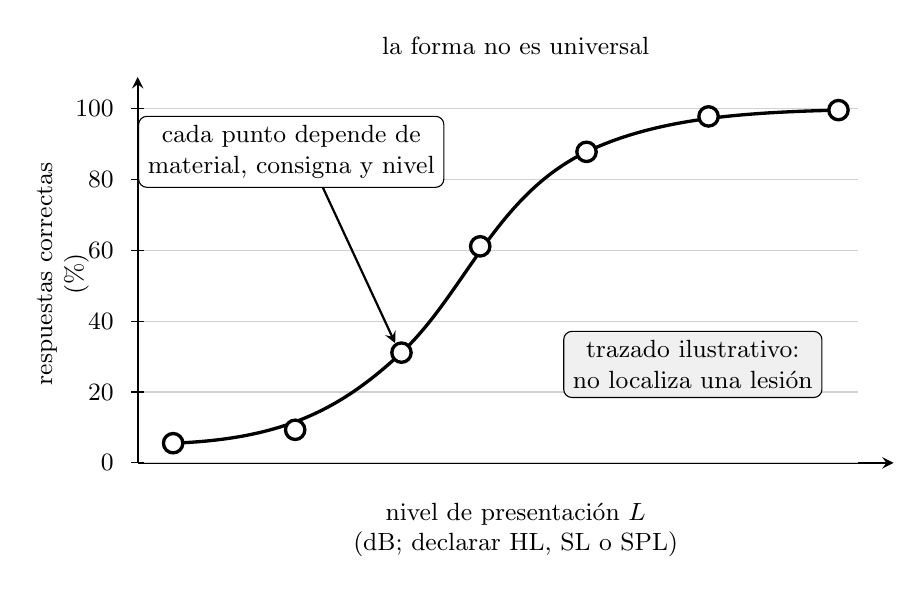
\begin{tikzpicture}[font=\small,>=stealth,x=1cm,y=1cm]
    \draw[->,thick] (1.20,0.80) -- (10.80,0.80);
    \draw[->,thick] (1.20,0.80) -- (1.20,5.70);
    \node[align=center] at (6.00,-0.05)
        {nivel de presentación \(L\)\\
         (\(\mathrm{dB}\); declarar HL, SL o SPL)};
    \node[rotate=90,align=center] at (0.25,3.20)
        {respuestas correctas\\(\(\%\))};

    \foreach \y/\lab in {0.80/0,1.70/20,2.60/40,3.50/60,4.40/80,5.30/100}{
        \draw[black!18] (1.20,\y) -- (10.35,\y);
        \draw (1.12,\y) -- (1.28,\y);
        \node[anchor=east] at (1.02,\y) {\lab};
    }

    \draw[very thick]
        (1.65,1.05)
        .. controls (3.00,1.10) and (3.75,1.45) .. (4.55,2.20)
        .. controls (5.35,2.95) and (5.75,4.20) .. (6.90,4.75)
        .. controls (7.80,5.18) and (8.90,5.25) .. (10.10,5.28);

    \foreach \x/\y in {
        1.65/1.05,3.20/1.22,4.55/2.20,5.55/3.55,
        6.90/4.75,8.45/5.20,10.10/5.28}{
        \fill[white] (\x,\y) circle (3.5pt);
        \draw[very thick] (\x,\y) circle (3.5pt);
    }

    \node[draw,rounded corners=3pt,fill=white,align=center]
        at (3.15,4.75)
        {cada punto depende de\\
         material, consigna y nivel};
    \draw[->,thick] (3.55,4.30) -- (4.47,2.32);

    \node[draw,rounded corners=3pt,fill=black!6,align=center]
        at (8.25,2.05)
        {trazado ilustrativo:\\
         no localiza una lesión};
    \node[align=center] at (6.00,6.10)
        {la forma no es universal};
\end{tikzpicture}

    \caption{Función desempeño--nivel de carácter conceptual. Cada punto
    relaciona un nivel de presentación, cuya escala debe declararse, con un
    porcentaje de respuestas correctas. La curva es ilustrativa: no procede
    de datos, no describe una lista verbal determinada y su forma aislada no
    localiza una lesión; elaboración propia.}
    \label{fig:u8-curva-logoaudiometrica}
\end{figure}

\subsection{Timpanometría}
\label{sec:u8-timpanometria}

\begin{description}[style=nextline]
    \item[Estímulo.]
    Un tono de sonda en el conducto auditivo mientras el equipo
    modifica la presión de aire en un intervalo controlado~\cite{ashaHearingAdults}.

    \item[Magnitud registrada.]
    Una magnitud de inmitancia acústica, habitualmente admitancia, en función
    de la presión del conducto. Deben declararse las unidades mostradas por el
    equipo; la presión suele expresarse en decapascales
    (\(\mathrm{daPa}\))~\cite{ashaHearingAdults}.

    \item[Parte del sistema evaluada.]
    La transferencia mecanoacústica dominada por el oído medio,
    condicionada también por el sellado de la sonda y el conducto~\cite{ashaHearingAdults}.

    \item[Respuesta conductual.]
    No requiere una respuesta voluntaria, aunque el movimiento, la
    vocalización o un sellado inadecuado pueden alterar el registro~\cite{ashaHearingAdults}.

    \item[Resultado básico esperado.]
    Un timpanograma: curva de admitancia o de otra magnitud de
    inmitancia frente a presión. Las clasificaciones morfológicas en tipos A, B
    y C son descripciones simplificadas y sus criterios dependen de la edad,
    el tono de sonda y el protocolo~\cite{ashaHearingAdults}.

    \item[Limitaciones generales.]
    La curva no mide directamente la audición ni identifica de manera única
    una patología. Debe interpretarse junto con el volumen estimado del
    conducto, los reflejos cuando corresponda y otras pruebas~\cite{ashaHearingAdults}.
\end{description}

La figura~\ref{fig:u8-timpanogramas} permite comparar tres morfologías sin
asignarles una causa clínica.

\begin{figure}[htbp]
    \centering
    \resizebox{\textwidth}{!}{%
        % Propósito: enseñar a comparar morfologías de timpanogramas sin convertirlas
% en diagnósticos ni presentar límites normativos.
% Origen: definición de timpanograma de la sección
% \ref{sec:u8-timpanometria}. Curvas sintéticas normalizadas:
% Y_N(x)=0.15+0.85 exp[-((x-x_0)/0.65)^2] para los picos,
% con x_0=0 y x_0=-1.15; el trazado plano usa Y_N=0.25.
% La coordenada x es sólo una posición esquemática de presión y no se convierte
% en valores de daPa. No hay datos medidos, normas ni intervalos de referencia.
% Descripción accesible: tres paneles comparten un eje vertical de admitancia
% normalizada y un eje horizontal de presión en decapascales. El primero tiene
% un pico centrado, el segundo es plano y el tercero tiene un pico desplazado
% hacia presiones negativas. Una nota indica que la forma no identifica por sí
% sola una patología.
% Validación prevista: comprobar las funciones, la normalización, el sentido de
% la presión, las unidades y que ningún panel incluya valores normativos.
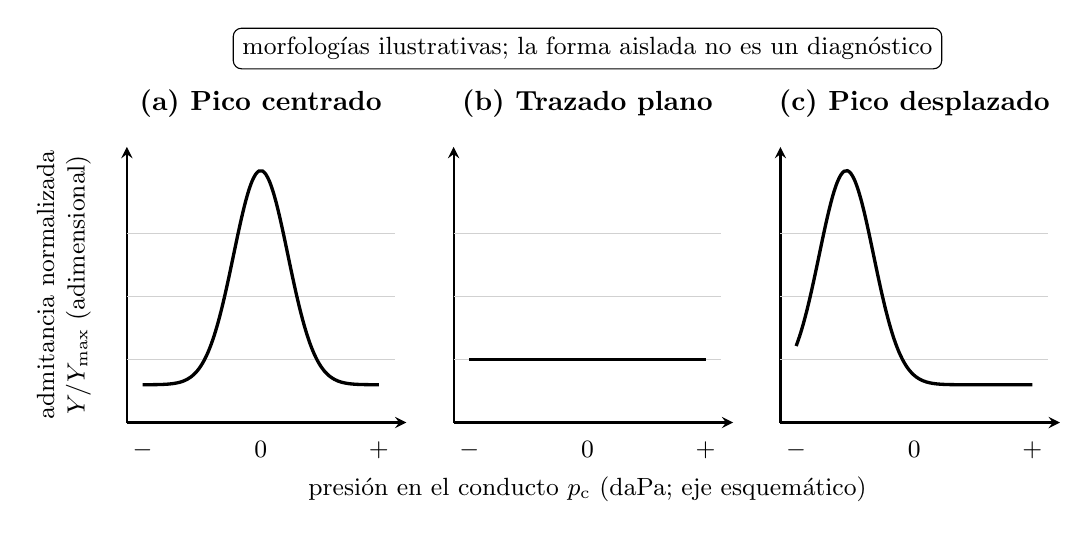
\begin{tikzpicture}[font=\small,>=stealth,x=1cm,y=1cm]
    \tikzset{
        axis/.style={->,thick},
        curve/.style={very thick},
        guide/.style={black!18,very thin}
    }

    \foreach \xshift/\title in {
        0/{(a) Pico centrado},
        4.15/{(b) Trazado plano},
        8.30/{(c) Pico desplazado}}{
        \begin{scope}[xshift=\xshift cm]
            \node[font=\bfseries] at (2.05,4.85) {\title};
            \draw[axis] (0.35,0.80) -- (3.90,0.80);
            \draw[axis] (0.35,0.80) -- (0.35,4.30);
            \draw[guide] (0.35,1.60) -- (3.75,1.60);
            \draw[guide] (0.35,2.40) -- (3.75,2.40);
            \draw[guide] (0.35,3.20) -- (3.75,3.20);
            \node[anchor=north] at (0.55,0.68) {\(-\)};
            \node[anchor=north] at (2.05,0.68) {\(0\)};
            \node[anchor=north] at (3.55,0.68) {\(+\)};
        \end{scope}
    }

    % x del gráfico = 2.05 + 0.75*u, con u en [-2,2].
    % y del gráfico = 0.80 + 3.20*Y_N.
    \draw[curve,domain=-2:2,samples=70,smooth,variable=\u]
        plot ({2.05+0.75*\u},{0.80+3.20*(0.15+0.85*exp(-(\u/0.65)^2))});
    \draw[curve] (4.70,1.60) -- (7.70,1.60);
    \draw[curve,domain=-2:2,samples=70,smooth,variable=\u]
        plot ({10.35+0.75*\u},{0.80+3.20*(0.15+0.85*exp(-((\u+1.15)/0.65)^2))});

    \node[rotate=90,align=center] at (-0.45,2.55)
        {admitancia normalizada\\\(Y/Y_{\max}\) (adimensional)};
    \node[align=center] at (6.20,-0.05)
        {presión en el conducto \(p_\mathrm{c}\)
         (\(\mathrm{daPa}\); eje esquemático)};
    \node[draw,rounded corners=3pt,fill=white,align=center]
        at (6.20,5.55)
        {morfologías ilustrativas; la forma aislada no es un diagnóstico};
\end{tikzpicture}
%
    }
    \caption{Morfologías esquemáticas de timpanogramas: pico centrado, trazado
    plano y pico desplazado hacia presiones negativas. La admitancia se
    normaliza respecto de su máximo y el eje de presión sólo indica sentido y
    unidad. Las curvas son funciones sintéticas, no datos medidos ni límites
    de referencia; una forma aislada no identifica una patología. Elaboración
    propia.}
    \label{fig:u8-timpanogramas}
    \label{fig:timpanometria}
\end{figure}

\subsection{Acufenometría}
\label{sec:u8-acufenometria}

\begin{description}[style=nextline]
    \item[Estímulo.]
    Tonos, ruidos de banda estrecha u otros sonidos ajustables en
    frecuencia y nivel~\cite{ashaTinnitus}.

    \item[Magnitud registrada.]
    La frecuencia de correspondencia en \(\mathrm{Hz}\), el nivel de
    correspondencia respecto del umbral en \(\mathrm{dB\,SL}\) y, según el
    protocolo, el nivel mínimo de enmascaramiento en decibeles con la escala
    indicada~\cite{ashaTinnitus}.

    \item[Parte del sistema evaluada.]
    La comparación perceptual entre el tinnitus referido y estímulos
    externos; no mide una fuente acústica interna~\cite{ashaTinnitus}.

    \item[Respuesta conductual.]
    Sí. La persona elige la alternativa que considera más parecida o
    informa cuándo se produce el efecto solicitado~\cite{ashaTinnitus}.

    \item[Resultado básico esperado.]
    Una caracterización psicoacústica de correspondencia. Los
    protocolos pueden incluir frecuencia, nivel, nivel mínimo de
    enmascaramiento e inhibición residual, con variabilidad entre sesiones~\cite{ashaTinnitus}.

    \item[Limitaciones generales.]
    El resultado depende de la consigna, del repertorio de estímulos y de la
    estabilidad perceptual. No cuantifica por sí solo el impacto funcional ni
    prescribe un tratamiento~\cite{ashaTinnitus}.
\end{description}

\subsection{Otoemisiones acústicas}
\label{sec:u8-oea}

\begin{description}[style=nextline]
    \item[Estímulo.]
    En las otoemisiones evocadas transitorias se emplean estímulos breves; en
    las otoemisiones por productos de distorsión se presentan dos tonos de
    frecuencias \(f_1\) y \(f_2\), expresadas en \(\mathrm{Hz}\)~\cite{ashaTinnitus}.

    \item[Magnitud registrada.]
    Presión sonora en el conducto auditivo mediante un micrófono de sonda. El
    equipo informa niveles de emisión y de ruido, en \(\mathrm{dB\,SPL}\), y
    relaciones señal--ruido en \(\mathrm{dB}\)~\cite{ashaHearingAdults}.

    \item[Parte del sistema evaluada.]
    El registro se asocia principalmente con la función de las células
    ciliadas externas, pero depende también de que el estímulo y la emisión
    atraviesen adecuadamente el oído externo y el oído medio~\cite{ashaHearingAdults}.

    \item[Respuesta conductual.]
    No requiere una respuesta voluntaria~\cite{ashaHearingAdults}.

    \item[Resultado básico esperado.]
    Emisión presente o ausente según criterios del protocolo, o amplitud por
    banda de frecuencia. En programas de pesquisa puede mostrarse una salida
    operativa del tipo ``pasa'' o ``derivar'', que no equivale a diagnóstico~\cite{ashaHearingAdults}.

    \item[Limitaciones generales.]
    El ruido, el ajuste de la sonda y el estado del oído externo y medio pueden
    impedir el registro. Una emisión presente no prueba una audición normal y
    una emisión ausente no localiza por sí sola una lesión~\cite{ashaHearingAdults}.
\end{description}

\subsection{Potenciales auditivos evocados}
\label{sec:u8-pea}

\begin{description}[style=nextline]
    \item[Estímulo.]
    Clics, ráfagas tonales o estímulos de banda más controlada,
    presentados a niveles y tasas definidos~\cite{ashaHearingAdults}.

    \item[Magnitud registrada.]
    Diferencias de potencial eléctrico registradas con electrodos de
    superficie, habitualmente en microvoltios (\(\mathrm{\mu V}\)), en
    función del tiempo posterior al estímulo, expresado en milisegundos
    (\(\mathrm{ms}\))~\cite{skinnerGlattke1977,ashaHearingAdults}.

    \item[Parte del sistema evaluada.]
    Los potenciales auditivos de tronco cerebral reflejan actividad
    neural sincronizada desde la porción distal del nervio auditivo y
    generadores del tronco encefálico. Otros potenciales auditivos exploran
    ventanas temporales y generadores diferentes~\cite{skinnerGlattke1977,ashaHearingAdults}.

    \item[Respuesta conductual.]
    No requiere una respuesta voluntaria. Sí requiere controlar
    impedancias de electrodos, artefactos, estado de reposo y calidad del
    promedio~\cite{skinnerGlattke1977,ashaHearingAdults}.

    \item[Resultado básico esperado.]
    Una forma de onda promediada con componentes identificables, latencias en
    \(\mathrm{ms}\) y amplitudes en \(\mathrm{\mu V}\), o una estimación
    de umbral según el protocolo~\cite{skinnerGlattke1977,ashaHearingAdults}.

    \item[Limitaciones generales.]
    La respuesta depende del estímulo, el nivel, la tasa, el estado fisiológico
    y el ruido eléctrico. Una respuesta neural no mide comprensión del habla y
    una estimación electrofisiológica no es idéntica a un umbral conductual~\cite{skinnerGlattke1977,ashaHearingAdults}.
\end{description}

\subsection{Electrococleografía}
\label{sec:u8-ecochg}

\begin{description}[style=nextline]
    \item[Estímulo.]
    Clics o ráfagas tonales presentados por vía aérea con parámetros
    controlados~\cite{skinnerGlattke1977,ashaHearingAdults}.

    \item[Magnitud registrada.]
    Potenciales eléctricos en microvoltios (\(\mathrm{\mu V}\)) y sus
    latencias en milisegundos (\(\mathrm{ms}\))~\cite{simpson2020}.

    \item[Parte del sistema evaluada.]
    La electrococleografía registra componentes asociados con la
    cóclea y la porción distal del nervio auditivo, entre ellos el potencial
    microfónico coclear, el potencial de sumación y el potencial de acción
    compuesto~\cite{simpson2020}.

    \item[Respuesta conductual.]
    No requiere una respuesta voluntaria~\cite{simpson2020}.

    \item[Resultado básico esperado.]
    Formas de onda y relaciones entre componentes definidas por el
    protocolo, no un rótulo diagnóstico automático~\cite{simpson2020}.

    \item[Limitaciones generales.]
    El electrodo puede colocarse por vía extratimpánica o
    transtimpánica; las técnicas difieren en invasividad y amplitud de señal.
    La utilidad diagnóstica y los criterios de interpretación dependen de la
    pregunta clínica y no son universales~\cite{simpson2020}.
\end{description}

\paragraph{OEA y potenciales: mediciones complementarias.}
La OEA registra una señal acústica en el conducto; un potencial evocado
registra una señal bioeléctrica mediante electrodos. Por lo tanto, una no
``confirma'' automáticamente a la otra~\cite{simpson2020}. Compararlas exige seguir la cadena
completa de estímulo, transmisión, generador, sensor, ruido y criterio de respuesta.

La figura~\ref{fig:u8-cadenas-oea-peat} hace visible por qué ambas pruebas no
son confirmaciones recíprocas: comparten una entrada acústica general, pero
registran magnitudes diferentes mediante sensores diferentes.

\begin{figure}[htbp]
    \centering
    \resizebox{\textwidth}{!}{%
        % Propósito: comparar qué estímulo ingresa, qué sensor registra la respuesta y
% qué magnitud informa una OEA frente a un PEAT.
% Origen: secciones \ref{sec:u8-oea}, \ref{sec:u8-pea} y párrafo
% "OEA y potenciales: mediciones complementarias". Esquema funcional sin
% tiempos, amplitudes, umbrales ni datos de pacientes.
% Descripción accesible: dos cadenas horizontales comienzan con un estímulo
% acústico. En la cadena OEA, una sonda emite el estímulo, el sonido atraviesa
% oído externo y medio, llega a la cóclea y una respuesta acústica regresa a un
% micrófono en el conducto; el resultado es presión o nivel y relación
% señal--ruido. En la cadena PEAT, un transductor entrega el estímulo, la
% actividad atraviesa cóclea, nervio y tronco; electrodos de superficie
% registran voltaje en microvoltios frente a tiempo en milisegundos.
% Validación prevista: comprobar la dirección de ida y retorno de OEA, que PEAT
% no muestre un micrófono como sensor, las unidades Pa/dB SPL/dB y microvoltios
% frente a milisegundos, que todos los bloques queden separados por flechas
% orientadas de manera inequívoca y la legibilidad al ancho de página.
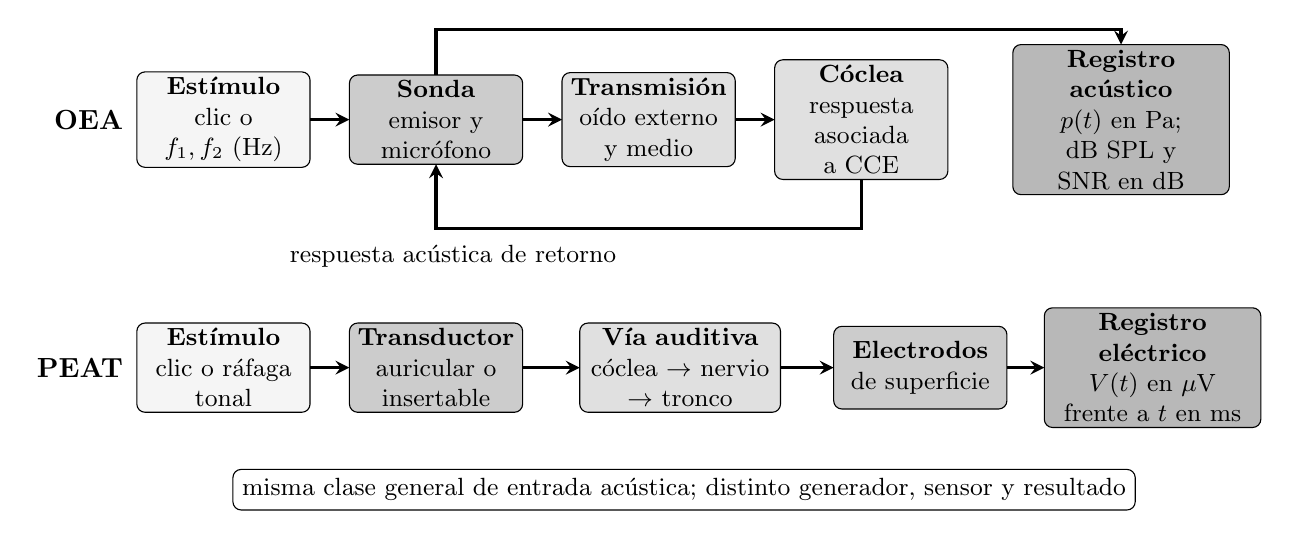
\begin{tikzpicture}[font=\small,>=stealth,x=1cm,y=1cm]
    \tikzset{
        block/.style={
            draw,rounded corners=3pt,
            text width=2.00cm,minimum width=2.20cm,minimum height=1.05cm,
            inner sep=2pt,outer sep=0pt,align=center
        },
        stimulus/.style={block,fill=black!4},
        pathway/.style={block,fill=black!12},
        sensor/.style={block,fill=black!20},
        result/.style={block,fill=black!28,text width=2.55cm,minimum width=2.75cm},
        flow/.style={->,very thick}
    }

    \node[font=\bfseries,anchor=east] at (0.00,4.40) {OEA};
    \node[stimulus] (oea-stim) at (1.15,4.40)
        {\textbf{Estímulo}\\clic o\\\(f_1,f_2\) (Hz)};
    \node[sensor] (probe) at (3.85,4.40)
        {\textbf{Sonda}\\emisor y\\micrófono};
    \node[pathway] (middle) at (6.55,4.40)
        {\textbf{Transmisión}\\oído externo\\y medio};
    \node[pathway] (cochlea) at (9.25,4.40)
        {\textbf{Cóclea}\\respuesta\\asociada a CCE};
    \node[result] (oea-out) at (12.55,4.40)
        {\textbf{Registro acústico}\\\(p(t)\) en Pa;\\dB SPL y SNR en dB};

    \draw[flow] (oea-stim.east) -- (probe.west);
    \draw[flow] (probe.east) -- (middle.west);
    \draw[flow] (middle.east) -- (cochlea.west);
    \draw[flow]
        (cochlea.south) -- ++(0,-0.62) -| (probe.south)
        node[pos=0.48,below=2pt] {respuesta acústica de retorno};
    \draw[flow] (probe.north) -- ++(0,0.58) -| (oea-out.north);

    \node[font=\bfseries,anchor=east] at (0.00,1.25) {PEAT};
    \node[stimulus] (abr-stim) at (1.15,1.25)
        {\textbf{Estímulo}\\clic o ráfaga\\tonal};
    \node[sensor] (earphone) at (3.85,1.25)
        {\textbf{Transductor}\\auricular o\\insertable};
    \node[pathway,text width=2.35cm,minimum width=2.55cm]
        (neural-path) at (6.95,1.25)
        {\textbf{Vía auditiva}\\cóclea \(\rightarrow\) nervio\\
         \(\rightarrow\) tronco};
    \node[sensor] (electrodes) at (10.00,1.25)
        {\textbf{Electrodos}\\de superficie};
    \node[result] (abr-out) at (12.95,1.25)
        {\textbf{Registro eléctrico}\\\(V(t)\) en \(\mathrm{\mu V}\)\\
         frente a \(t\) en \(\mathrm{ms}\)};

    \draw[flow] (abr-stim.east) -- (earphone.west);
    \draw[flow] (earphone.east) -- (neural-path.west);
    \draw[flow] (neural-path.east) -- (electrodes.west);
    \draw[flow] (electrodes.east) -- (abr-out.west);

    \node[draw,rounded corners=3pt,fill=white,align=center]
        at (7.00,-0.30)
        {misma clase general de entrada acústica; distinto generador,
         sensor y resultado};
\end{tikzpicture}
%
    }
    \caption{Comparación funcional de las cadenas de medición de OEA y PEAT.
    En OEA, una sonda presenta el estímulo y registra presión acústica de
    retorno en el conducto; en PEAT, electrodos de superficie registran una
    diferencia de potencial bioeléctrico en función del tiempo. El esquema no
    representa amplitudes, latencias, umbrales ni datos de pacientes;
    elaboración propia.}
    \label{fig:u8-cadenas-oea-peat}
\end{figure}

\section{Bloque III. Técnicas y dispositivos de rehabilitación}
\label{sec:u8-rehabilitacion}

Un dispositivo de rehabilitación transforma una señal; no borra la
alteración ni reproduce necesariamente la audición habitual. La
selección, adaptación y seguimiento dependen de la evaluación audiológica,
las necesidades comunicativas, la anatomía, las preferencias y el contexto de
cada persona, dentro de un equipo profesional~\cite{ashaHearingAdults,skinnerGlattke1977}.

\subsection{Audífonos}
\label{sec:u8-audifonos}

En su cadena funcional más simple, un micrófono convierte presión acústica en
señal eléctrica; un procesador modifica esa señal; y un receptor la convierte
nuevamente en sonido cerca del oído. El procesamiento puede depender de la
frecuencia, del nivel de entrada y del tiempo~\cite{whoHearing2021}.

Sea \(L_{\mathrm{ent}}(f)\) el nivel de presión sonora de entrada y
\(L_{\mathrm{sal}}(f)\) el nivel de presión sonora de salida, ambos en
\(\mathrm{dB\,SPL}\), para la frecuencia \(f\) en \(\mathrm{Hz}\). La
ganancia electroacústica es:

\begin{equation}
    G(f)=L_{\mathrm{sal}}(f)-L_{\mathrm{ent}}(f),
    \label{eq:u8-ganancia}
\end{equation}

donde \(G(f)\) se expresa en \(\mathrm{dB}\). Con datos ficticios, una entrada
de \(52\,\mathrm{dB\,SPL}\) y una salida de
\(70\,\mathrm{dB\,SPL}\) a \(2000\,\mathrm{Hz}\) corresponden a
una ganancia de \(18\,\mathrm{dB}\) en esa condición. Este cálculo no
determina una prescripción.

Los audífonos actuales pueden incluir compresión dependiente del
nivel, micrófonos direccionales, reducción de ruido y control de
realimentación. Su efecto depende de la adaptación, del ambiente y de las
características de la señal; no existe una ganancia fija adecuada para todas
las personas~\cite{whoHearing2021}.

\subsection{Implantes cocleares}
\label{sec:u8-implantes}

El implante coclear cambia la naturaleza de la señal dentro de la cadena. Un
micrófono capta sonido; el procesador extrae y codifica información; un enlace
transmite los datos al receptor--estimulador implantado; y una guía de
electrodos entrega pulsos eléctricos en la cóclea~\cite{nidcdCI2024}.

El objetivo es estimular poblaciones neurales auditivas evitando que
la transducción dependa exclusivamente de las células sensoriales dañadas. La
cantidad de electrodos físicos, la cantidad de canales programados y la
cantidad de bandas perceptualmente independientes no son magnitudes
equivalentes~\cite{nidcdCI2024}.

Un implante no es un audífono de mayor potencia: el audífono mantiene
una salida acústica, mientras que el implante produce estimulación eléctrica~\cite{nidcdCI2024}.
Los criterios de candidatura y los resultados esperables cambian con
la edad, la historia auditiva, la anatomía, el acceso al lenguaje y las guías
clínicas vigentes; no deben reducirse a un porcentaje universal de
reconocimiento verbal~\cite{nidcdCI2024}.

\subsection{Dispositivos de conducción ósea}
\label{sec:u8-conduccion-osea}

Estos dispositivos convierten una señal eléctrica en vibración mecánica
aplicada al cráneo. La vibración se transmite por varios mecanismos de
conducción ósea y puede estimular ambas cócleas en distinta proporción. No es
correcto decir que la energía viaja sólo a la cóclea del lado estimulado~\cite{stenfeltGoode2005,whoHearing2021}.

Existen configuraciones externas, percutáneas y transcutáneas, con
indicaciones y limitaciones diferentes. Pueden considerarse en determinadas
alteraciones conductivas, mixtas o unilaterales, pero la elección requiere
evaluación individual y no se deduce de la etiqueta diagnóstica aislada~\cite{stenfeltGoode2005,whoHearing2021}.

\subsection{Estimulación electroacústica}
\label{sec:u8-eas}

Este sistema combina una salida acústica y otra eléctrica en un mismo oído~\cite{nidcdCI2024,whoHearing2021}.
Puede emplearse cuando existe audición
residual útil en una región frecuencial y se busca aportar estimulación
eléctrica en otra. La frecuencia de separación no es fija: depende de los
umbrales, del dispositivo, de la programación y de la evolución individual~\cite{nidcdCI2024,whoHearing2021}.

\begin{table}[htbp]
    \centering
    \caption{Comparación física de dispositivos de rehabilitación. La tabla
    describe transformaciones de señal, no indicaciones clínicas.}
    \label{tab:u8-dispositivos}
    \small
    \setlength{\tabcolsep}{3pt}
    \begin{tabular}{
        >{\raggedright\arraybackslash}p{0.20\textwidth}
        >{\raggedright\arraybackslash}p{0.24\textwidth}
        >{\raggedright\arraybackslash}p{0.22\textwidth}
        >{\raggedright\arraybackslash}p{0.24\textwidth}}
        \hline
        \textbf{Dispositivo} & \textbf{Entrada y procesamiento} &
        \textbf{Salida principal} & \textbf{Límite conceptual} \\
        \hline
        Audífono &
        Sonido \(\rightarrow\) señal eléctrica procesada &
        Sonido en el conducto &
        Amplificar no restaura automáticamente resolución ni comprensión. \\
        Implante coclear &
        Sonido \(\rightarrow\) código de estimulación &
        Pulsos eléctricos en la cóclea &
        Electrodos, canales y bandas perceptuales no son equivalentes. \\
        Conducción ósea &
        Sonido \(\rightarrow\) señal eléctrica procesada &
        Vibración mecánica del cráneo &
        La transmisión alcanza ambas cócleas y depende del acoplamiento. \\
        Electroacústico &
        Procesamiento acústico y eléctrico combinado &
        Sonido y pulsos eléctricos &
        La división frecuencial debe individualizarse. \\
        \hline
    \end{tabular}
\end{table}

La figura~\ref{fig:u8-cadenas-dispositivos} completa la tabla al localizar el
punto en que cambia la naturaleza física de la señal.

\begin{figure}[htbp]
    \centering
    \resizebox{\textwidth}{!}{%
        % Propósito: distinguir las transformaciones físicas de audífono, implante
% coclear y dispositivo de conducción ósea.
% Origen: secciones \ref{sec:u8-audifonos}, \ref{sec:u8-implantes} y
% \ref{sec:u8-conduccion-osea}, más la notación de presión p(t), corriente i(t)
% y desplazamiento xi(t). Esquema funcional; no representa marcas, anatomía,
% estrategias de codificación, ganancias ni indicaciones clínicas.
% Descripción accesible: tres filas parten de presión acústica en pascales y
% pasan por micrófono y procesamiento eléctrico. El audífono usa un receptor y
% vuelve a producir presión acústica cerca del oído. El implante usa un enlace,
% estimulador y electrodos para producir corriente eléctrica en la cóclea. El
% dispositivo de conducción ósea usa un vibrador para producir desplazamiento
% mecánico en el cráneo. Los sombreados separan dominios acústico, eléctrico y
% mecánico.
% Validación prevista: comprobar que las tres entradas son acústicas, que las
% salidas se expresan como p(t) en Pa, i(t) en A y xi(t) en m, que el implante
% no aparece como amplificador acústico, que la vía ósea no se dibuja hacia
% una única cóclea y que las flechas conserven una separación visible entre
% bloques al ancho final de página.
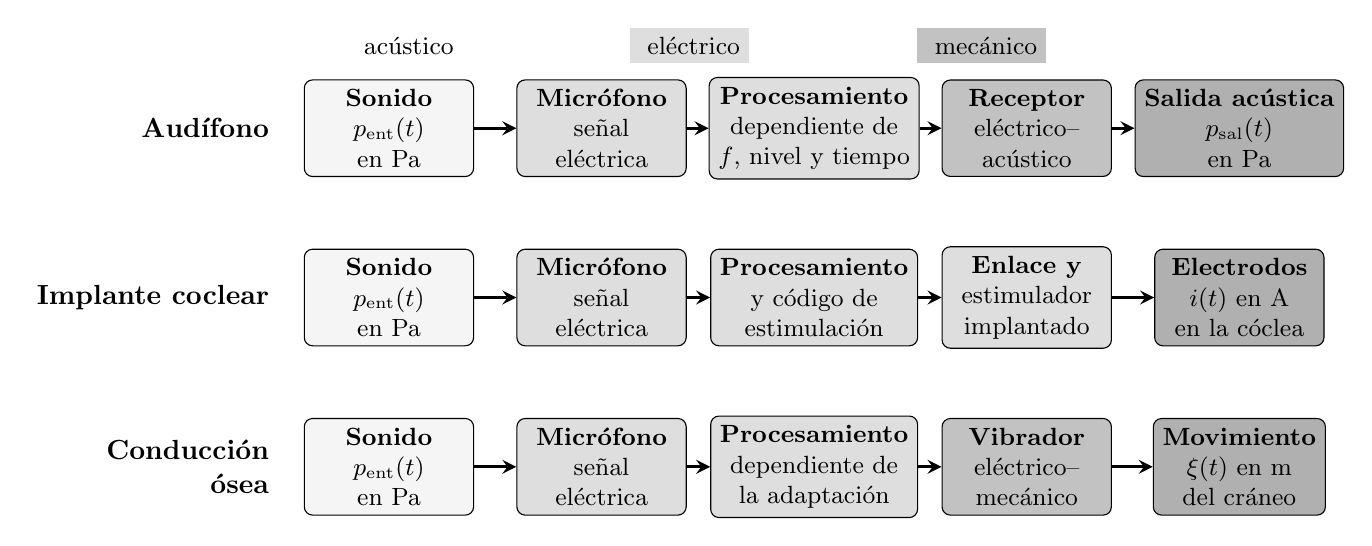
\begin{tikzpicture}[font=\small,>=stealth,x=1cm,y=1cm]
    \tikzset{
        block/.style={
            draw,rounded corners=3pt,
            minimum width=2.15cm,minimum height=1.05cm,
            align=center
        },
        acoustic/.style={block,fill=black!4},
        electric/.style={block,fill=black!13},
        mechanical/.style={block,fill=black!24},
        output/.style={block,fill=black!31},
        flow/.style={->,very thick}
    }

    \node[font=\bfseries,anchor=east] at (0.15,5.10) {Audífono};
    \node[acoustic] (ha-in) at (1.55,5.10)
        {\textbf{Sonido}\\\(p_\mathrm{ent}(t)\)\\en Pa};
    \node[electric] (ha-mic) at (4.25,5.10)
        {\textbf{Micrófono}\\señal\\eléctrica};
    \node[electric] (ha-proc) at (6.95,5.10)
        {\textbf{Procesamiento}\\dependiente de\\\(f\), nivel y tiempo};
    \node[mechanical] (ha-rec) at (9.65,5.10)
        {\textbf{Receptor}\\eléctrico--\\acústico};
    \node[output] (ha-out) at (12.35,5.10)
        {\textbf{Salida acústica}\\\(p_\mathrm{sal}(t)\)\\en Pa};

    \node[font=\bfseries,anchor=east] at (0.15,2.95) {Implante coclear};
    \node[acoustic] (ci-in) at (1.55,2.95)
        {\textbf{Sonido}\\\(p_\mathrm{ent}(t)\)\\en Pa};
    \node[electric] (ci-mic) at (4.25,2.95)
        {\textbf{Micrófono}\\señal\\eléctrica};
    \node[electric] (ci-proc) at (6.95,2.95)
        {\textbf{Procesamiento}\\y código de\\estimulación};
    \node[electric] (ci-link) at (9.65,2.95)
        {\textbf{Enlace y}\\estimulador\\implantado};
    \node[output] (ci-out) at (12.35,2.95)
        {\textbf{Electrodos}\\\(i(t)\) en A\\en la cóclea};

    \node[font=\bfseries,anchor=east,align=right] at (0.15,0.80)
        {Conducción\\ósea};
    \node[acoustic] (bc-in) at (1.55,0.80)
        {\textbf{Sonido}\\\(p_\mathrm{ent}(t)\)\\en Pa};
    \node[electric] (bc-mic) at (4.25,0.80)
        {\textbf{Micrófono}\\señal\\eléctrica};
    \node[electric] (bc-proc) at (6.95,0.80)
        {\textbf{Procesamiento}\\dependiente de\\la adaptación};
    \node[mechanical] (bc-vib) at (9.65,0.80)
        {\textbf{Vibrador}\\eléctrico--\\mecánico};
    \node[output] (bc-out) at (12.35,0.80)
        {\textbf{Movimiento}\\\(\xi(t)\) en m\\del cráneo};

    \foreach \a/\b in {
        ha-in/ha-mic,ha-mic/ha-proc,ha-proc/ha-rec,ha-rec/ha-out,
        ci-in/ci-mic,ci-mic/ci-proc,ci-proc/ci-link,ci-link/ci-out,
        bc-in/bc-mic,bc-mic/bc-proc,bc-proc/bc-vib,bc-vib/bc-out}{
        \draw[flow] (\a.east) -- (\b.west);
    }

    \node[anchor=west] at (1.00,6.15)
        {\(\square\) acústico};
    \node[anchor=west,fill=black!13] at (4.60,6.15)
        {\(\square\) eléctrico};
    \node[anchor=west,fill=black!24] at (8.25,6.15)
        {\(\square\) mecánico};
\end{tikzpicture}
%
    }
    \caption{Transformaciones físicas principales en tres dispositivos. El
    audífono vuelve a producir presión acústica cerca del oído; el implante
    coclear entrega estimulación eléctrica mediante electrodos; y el
    dispositivo de conducción ósea produce movimiento mecánico del cráneo.
    Las variables y unidades identifican dominios físicos, no formas de onda,
    ganancias, marcas comerciales ni indicaciones clínicas. Esquema
    funcional, sin escala; elaboración propia.}
    \label{fig:u8-cadenas-dispositivos}
\end{figure}

\section{Relación con la Fonoaudiología}
\label{sec:u8-relacion-fonoaudiologia}

El aporte de la física acústica consiste en hacer explícita la cadena de
medición o transformación:

\begin{enumerate}
    \item identificar qué energía ingresa y con qué unidades se describe;
    \item reconocer qué estructura o función modifica esa energía;
    \item establecer qué sensor o respuesta produce el dato;
    \item distinguir el dato físico del juicio perceptual;
    \item declarar qué conclusiones permite el procedimiento y cuáles no.
\end{enumerate}

Esta secuencia ayuda a evitar dos extremos: atribuir a una prueba más alcance
del que posee y tratar los dispositivos como soluciones intercambiables.
En la práctica profesional, la evaluación auditiva se construye con
una batería seleccionada según la edad, la consulta y las condiciones de
respuesta; la interpretación integrada corresponde a profesionales
habilitados y a protocolos vigentes~\cite{ashaHearingAdults}.

\section{Errores frecuentes y advertencias}
\label{sec:u8-errores}

\begin{description}[style=nextline]
    \item[``TTS y tinnitus son lo mismo''.]
    El TTS es una diferencia entre umbrales medidos; el tinnitus es una
    percepción referida.

    \item[``Una escotadura demuestra daño por ruido''.]
    Describe una forma del audiograma, pero no demuestra una causa.

    \item[``dB SPL y dB HL pueden restarse sin más''.]
    Utilizan referencias diferentes. Sólo deben combinarse magnitudes
    compatibles y con la escala declarada.

    \item[``La timpanometría mide cuánto oye una persona''.]
    Registra una magnitud de inmitancia frente a presión; no es una medición
    directa del umbral.

    \item[``Una OEA presente demuestra audición normal''.]
    Informa sobre una parte de la cadena y no evalúa por sí sola la respuesta
    neural, perceptual o lingüística.

    \item[``Un potencial evocado mide comprensión del habla''.]
    Registra una respuesta bioeléctrica sincronizada, no desempeño
    comunicativo.

    \item[``La frecuencia de acufenometría es la frecuencia física del
    tinnitus''.]
    Es una correspondencia perceptual con un estímulo externo.

    \item[``Un tipo de timpanograma equivale a una enfermedad''.]
    La morfología es un dato que requiere integración con otras observaciones.

    \item[``Un audífono devuelve una audición normal''.]
    Modifica la señal acústica, pero no elimina todas las limitaciones del
    sistema auditivo ni del ambiente.

    \item[``Más electrodos implican la misma cantidad de frecuencias
    independientes''.]
    Electrodos físicos, canales de procesamiento y perceptos independientes
    son conceptos distintos.

    \item[``La conducción ósea estimula solamente un oído''.]
    La vibración del cráneo puede alcanzar ambas cócleas.

    \item[``Una sola prueba alcanza para diagnosticar e indicar un
    dispositivo''.]
    Cada prueba responde a una pregunta limitada; la decisión profesional
    integra varias fuentes de información.
\end{description}

\section{Síntesis}
\label{sec:u8-sintesis}

\begin{itemize}
    \item El primer bloque separó exposición, alteración, síntoma y resultado.
    El TTS se definió como una diferencia de umbrales; la PAIR, el trauma
    acústico, el tinnitus, la presbiacusia y la ototoxicidad se presentaron
    sin umbrales causales ni tratamientos universales.
    \item El segundo bloque comparó estudios mediante seis preguntas comunes:
    estímulo, magnitud, parte del sistema, respuesta conductual, resultado y
    limitaciones. Una prueba conductual y una fisiológica producen datos
    diferentes y complementarios.
    \item El tercer bloque describió transformaciones físicas. El audífono
    entrega sonido, el implante coclear entrega pulsos eléctricos y el
    dispositivo de conducción ósea entrega vibración mecánica.
    \item Un registro aislado no equivale a un diagnóstico. La interpretación
    exige declarar escalas, unidades, condiciones de medición y alcance.
\end{itemize}

\section{Ejercicios y autoevaluación}
\label{sec:u8-ejercicios}

\subsection*{Preguntas conceptuales}

\begin{enumerate}[label=\textbf{C\arabic*.},leftmargin=*]
    \item Una persona percibe tinnitus después de una exposición. Explique por
    qué esa percepción no demuestra que exista TTS.

    \item En un registro ficticio se informa una exposición de
    \(L_{A\mathrm{eq},2\,\mathrm{h}}=90\,\mathrm{dB(A)}\), tinnitus referido y un umbral
    de \(40\,\mathrm{dB\,HL}\) a \(4000\,\mathrm{Hz}\). Clasifique esos tres
    datos como exposición, síntoma o resultado de medición. Explique por qué
    ninguno demuestra por sí solo una alteración determinada.

    \item ¿Por qué una escotadura audiométrica no alcanza para afirmar que la
    causa es una exposición laboral a ruido?

    \item Compare una prueba conductual con una fisiológica. Mencione una
    ventaja y una limitación de cada enfoque.

    \item Explique por qué una OEA ausente y un potencial evocado presente no
    son resultados necesariamente contradictorios.

    \item ¿Qué diferencia existe entre el nivel físico de un tono de
    comparación y la sonoridad del tinnitus referido?

    \item Compare las salidas físicas de un audífono, un implante coclear y un
    dispositivo de conducción ósea.

    \item ¿Por qué ``más ganancia'' no significa necesariamente ``mejor
    comprensión''?
\end{enumerate}

\subsection*{Identificación e interpretación de gráficos}

\begin{enumerate}[label=\textbf{G\arabic*.},leftmargin=*]
    \item Observe la Figura~\ref{fig:u8-audiograma-conceptual}.
    \begin{enumerate}
        \item Identifique la magnitud y la unidad de cada eje, e indique hacia
        dónde aumenta el nivel de audición.
        \item Lea los valores ficticios de vía aérea y vía ósea a
        \(1000\,\mathrm{Hz}\).
        \item Calcule \(G_{\mathrm{AO}}\) en esa frecuencia.
        \item Escriba una conclusión que la figura no permite formular.
    \end{enumerate}

    \item En la Figura~\ref{fig:u8-curva-logoaudiometrica}, identifique la
    variable de cada eje. Explique por qué no pueden leerse valores absolutos
    del eje horizontal sin declarar si el nivel se expresa en
    \(\mathrm{dB\,HL}\), \(\mathrm{dB\,SL}\) o \(\mathrm{dB\,SPL}\), y por qué
    la curva no localiza por sí sola una lesión.

    \item Compare los tres paneles de la
    Figura~\ref{fig:u8-timpanogramas}. Identifique el pico centrado, el trazado
    plano y el pico desplazado hacia presiones negativas. Indique qué
    representa \(Y/Y_{\max}\), qué unidad posee la presión y qué interpretación
    clínica no puede realizarse a partir de la forma aislada.

    \item Recorra la fila OEA de la
    Figura~\ref{fig:u8-cadenas-oea-peat}. Identifique el estímulo, el trayecto
    de ida, el trayecto de retorno, el sensor y las magnitudes de salida con
    sus unidades.

    \item Recorra la fila PEAT de la
    Figura~\ref{fig:u8-cadenas-oea-peat}. Identifique qué parte de la cadena
    sigue siendo acústica, dónde se genera la respuesta bioeléctrica, qué
    sensor la registra y por qué el resultado no mide comprensión del habla.

    \item En la Figura~\ref{fig:u8-cadenas-dispositivos}, marque en cada fila el
    punto en que cambia el dominio físico de la señal. Compare las salidas
    \(p_{\mathrm{sal}}(t)\) en \(\mathrm{Pa}\), \(i(t)\) en
    \(\mathrm{A}\) y \(\xi(t)\) en \(\mathrm{m}\), sin asignar una indicación
    clínica al dispositivo.
\end{enumerate}

\subsection*{Ejercicios numéricos guiados}

\begin{enumerate}[label=\textbf{NG\arabic*.},leftmargin=*]
    \item A \(4000\,\mathrm{Hz}\), un umbral de referencia ficticio es
    \(L_{\mathrm{U},0}=12\,\mathrm{dB\,HL}\). A los
    \(\Delta t=30\,\mathrm{min}\) se mide
    \(L_{\mathrm{U},1}=27\,\mathrm{dB\,HL}\).
    \begin{enumerate}
        \item Verifique que ambos datos poseen la misma escala y corresponden a
        la misma frecuencia.
        \item Escriba la Ecuación~\eqref{eq:u8-tts} y sustituya los valores.
        \item Calcule \(\Delta L_{\mathrm{T}}\) en \(\mathrm{dB}\).
        \item Interprete el signo sin atribuir una causa ni una permanencia.
    \end{enumerate}

    \item Una fuente aporta \(L_{A\mathrm{eq},2\,\mathrm{h}}=92\,\mathrm{dB(A)}\)
    durante dos horas y su contribución es despreciable durante las otras seis.
    \begin{enumerate}
        \item Calcule el cociente adimensional
        \((2\,\mathrm{h})/(8\,\mathrm{h})\).
        \item Aplique la normalización temporal empleada en
        \eqref{eq:u8-leq-ejemplo}.
        \item Exprese \(L_{A\mathrm{eq},8\,\mathrm{h}}\) con una cifra decimal.
        \item Indique qué conclusión normativa no puede extraerse.
    \end{enumerate}

    \item Con datos didácticos ficticios, a \(2000\,\mathrm{Hz}\) se obtiene
    \(L_{\mathrm{VA}}=45\,\mathrm{dB\,HL}\) y
    \(L_{\mathrm{VO}}=15\,\mathrm{dB\,HL}\). Calcule
    \(G_{\mathrm{AO}}\) siguiendo estos pasos: compruebe la compatibilidad de
    escalas, aplique \eqref{eq:u8-gap}, conserve la unidad
    \(\mathrm{dB}\) en el resultado y limite su interpretación.

    \item A \(1000\,\mathrm{Hz}\), un audífono recibe y entrega,
    respectivamente,
    \[
        L_{\mathrm{ent}}=50\,\mathrm{dB\,SPL}
        \quad\text{y}\quad
        L_{\mathrm{sal}}=68\,\mathrm{dB\,SPL}.
    \]
    Verifique que ambos niveles usan la misma referencia, aplique
    \eqref{eq:u8-ganancia}, calcule la ganancia en \(\mathrm{dB}\) e indique
    qué dato comunicativo no proporciona el resultado.
\end{enumerate}

\subsection*{Ejercicios numéricos autónomos}

\begin{enumerate}[label=\textbf{NA\arabic*.},leftmargin=*]
    \item Los siguientes umbrales ficticios se obtienen antes de una
    exposición y a los \(\Delta t=45\,\mathrm{min}\):
    \[
    \begin{array}{c|ccc}
        f\;(\mathrm{Hz}) & 500 & 1000 & 4000 \\ \hline
        L_{\mathrm{U},0}\;(\mathrm{dB\,HL}) & 10 & 15 & 20 \\
        L_{\mathrm{U},1}\;(\mathrm{dB\,HL}) & 16 & 28 & 31
    \end{array}
    \]
    Calcule \(\Delta L_{\mathrm{T}}\) para cada frecuencia, identifique la
    mayor diferencia medida y explique por qué la tabla no determina su causa
    ni su evolución posterior.

    \item Una fuente aporta \(L_{A\mathrm{eq},0{,}5\,\mathrm{h}}=96\,\mathrm{dB(A)}\)
    durante \(0{,}5\,\mathrm{h}\), y su contribución durante las otras
    \(7{,}5\,\mathrm{h}\) es despreciable. Calcule
    \(L_{A\mathrm{eq},8\,\mathrm{h}}\) y redondee el resultado a una cifra decimal.

    \item Para un audífono se obtienen los siguientes niveles ficticios:
    \[
    \begin{array}{c|ccc}
        f\;(\mathrm{Hz}) & 500 & 1000 & 2000 \\ \hline
        L_{\mathrm{ent}}\;(\mathrm{dB\,SPL}) & 54 & 54 & 54 \\
        L_{\mathrm{sal}}\;(\mathrm{dB\,SPL}) & 64 & 69 & 75
    \end{array}
    \]
    Calcule \(G(f)\) en cada frecuencia, identifique dónde es mayor y explique
    qué atributo perceptual o desempeño comunicativo no puede deducirse de
    esos tres valores.

    \item Un audiograma ficticio contiene:
    \[
    \begin{array}{c|ccc}
        f\;(\mathrm{Hz}) & 500 & 1000 & 4000 \\ \hline
        L_{\mathrm{VA}}\;(\mathrm{dB\,HL}) & 25 & 40 & 55 \\
        L_{\mathrm{VO}}\;(\mathrm{dB\,HL}) & 10 & 15 & 30
    \end{array}
    \]
    Calcule \(G_{\mathrm{AO}}(f)\) para cada frecuencia e identifique si existe
    una única diferencia máxima. No asigne un diagnóstico al patrón.
\end{enumerate}

\subsection*{Aplicaciones en Fonoaudiología}

\begin{enumerate}[label=\textbf{A\arabic*.},leftmargin=*]
    \item Para cada una de las siguientes preguntas de medición, asigne el
    estudio más directamente relacionado, indique si requiere respuesta
    conductual y escriba la magnitud principal con su unidad:
    \begin{enumerate}
        \item umbral auditivo en función de la frecuencia \(f\), expresada en
        \(\mathrm{Hz}\);
        \item desempeño ante material verbal;
        \item transferencia mecanoacústica dominada por el oído medio;
        \item correspondencia perceptual con un tinnitus referido;
        \item respuesta acústica asociada con función coclear;
        \item respuesta bioeléctrica sincronizada del nervio y el tronco;
        \item potenciales cocleares y de la porción distal del nervio.
    \end{enumerate}

    \item Un informe logoaudiométrico sólo consigna ``72\,\% de respuestas
    correctas''. Enumere al menos cinco datos que deben acompañar ese
    porcentaje para que pueda interpretarse dentro del alcance de esta unidad.

    \item En una medición timpanométrica aparece un trazado plano. Escriba dos
    conclusiones que no pueden extraerse de ese único dato y tres condiciones
    técnicas o complementarias que deben revisarse antes de interpretarlo.

    \item Una pesquisa mediante OEA informa ``derivar''. Redacte una
    explicación breve que diferencie esa salida operativa de un diagnóstico y
    mencione tres factores técnicos o de transmisión que pueden afectar el
    registro.

    \item Tres dispositivos sin identificar producen, respectivamente:
    presión acústica \(p_{\mathrm{sal}}(t)\) en \(\mathrm{Pa}\) cerca del oído,
    corriente \(i(t)\) en \(\mathrm{A}\) mediante electrodos cocleares y
    desplazamiento \(\xi(t)\) en \(\mathrm{m}\) del cráneo. Identifique el
    audífono, el implante coclear y el dispositivo de conducción ósea. Explique
    por qué esta identificación física no basta para seleccionar uno para una
    persona.
\end{enumerate}

\subsection*{Pregunta integradora}

\begin{enumerate}[label=\textbf{INT\arabic*.},leftmargin=*]
    \item Considere el siguiente caso didáctico ficticio:
    \begin{itemize}
        \item durante \(1\,\mathrm{h}\) se registra
        \(L_{A\mathrm{eq},1\,\mathrm{h}}=94\,\mathrm{dB(A)}\), con contribución
        despreciable durante las otras \(7\,\mathrm{h}\);
        \item la persona refiere tinnitus y selecciona un tono de
        \(6000\,\mathrm{Hz}\) a \(8\,\mathrm{dB\,SL}\) como correspondencia;
        \item a \(4000\,\mathrm{Hz}\), el umbral de referencia es
        \(15\,\mathrm{dB\,HL}\) y a los \(\Delta t=45\,\mathrm{min}\) se mide
        \(30\,\mathrm{dB\,HL}\);
        \item una pesquisa mediante OEA informa ``derivar''.
    \end{itemize}
    \begin{enumerate}
        \item Clasifique cada dato como descriptor de exposición, respuesta
        perceptual, resultado conductual o resultado fisiológico.
        \item Calcule \(L_{A\mathrm{eq},8\,\mathrm{h}}\) con una cifra decimal.
        \item Calcule \(\Delta L_{\mathrm{T}}\) a \(4000\,\mathrm{Hz}\).
        \item Explique por qué \(6000\,\mathrm{Hz}\) y
        \(8\,\mathrm{dB\,SL}\) no describen una fuente física interna.
        \item Indique dos preguntas que permanecen abiertas y asigne a cada una
        un estudio de esta unidad, sin formular un diagnóstico ni un
        tratamiento.
    \end{enumerate}
\end{enumerate}

\subsection*{Errores frecuentes y distractores razonables}

\begin{enumerate}[label=\textbf{D\arabic*.},leftmargin=*]
    \item Seleccione la afirmación correcta:
    \begin{enumerate}
        \item La timpanometría mide umbrales en \(\mathrm{dB\,HL}\).
        \item La audiometría tonal requiere una respuesta conductual.
        \item La OEA registra voltaje mediante electrodos.
        \item La acufenometría mide una fuente acústica dentro del oído.
    \end{enumerate}

    \item Seleccione la afirmación correcta:
    \begin{enumerate}
        \item Un audífono entrega estimulación eléctrica intracoclear.
        \item Un implante coclear sólo aumenta la presión sonora.
        \item Un dispositivo de conducción ósea entrega vibración mecánica.
        \item Todos los dispositivos producen la misma salida física.
    \end{enumerate}

    \item Seleccione la afirmación correcta sobre las figuras de esta unidad:
    \begin{enumerate}
        \item El eje vertical del audiograma expresa
        \(\mathrm{dB\,SPL}\).
        \item Un trazado timpanométrico plano identifica por sí solo una
        enfermedad.
        \item OEA y PEAT utilizan el mismo sensor y registran la misma
        magnitud.
        \item La Figura~\ref{fig:u8-cadenas-dispositivos} distingue dominios
        acústico, eléctrico y mecánico.
    \end{enumerate}

    \item Seleccione la operación físicamente válida:
    \begin{enumerate}
        \item Restar \(70\,\mathrm{dB\,SPL}-50\,\mathrm{dB\,HL}\) para obtener
        una ganancia de \(20\,\mathrm{dB}\).
        \item Comparar dos umbrales en \(\mathrm{dB\,HL}\), medidos a la misma
        frecuencia y en tiempos diferentes, para calcular
        \(\Delta L_{\mathrm{T}}\).
        \item Interpretar \(8\,\mathrm{dB\,SL}\) como la intensidad física del
        tinnitus.
        \item Expresar un porcentaje logoaudiométrico en
        \(\mathrm{dB\,SPL}\).
    \end{enumerate}

    \item Ante un valor \(\Delta L_{\mathrm{T}}=15\,\mathrm{dB}\) a
    \(4000\,\mathrm{Hz}\), seleccione la conclusión compatible con el alcance
    de la unidad:
    \begin{enumerate}
        \item demuestra una PAIR permanente;
        \item demuestra la presencia de tinnitus;
        \item describe una diferencia positiva entre dos umbrales obtenidos en
        esas condiciones;
        \item establece que la exposición cumplió una norma.
    \end{enumerate}
\end{enumerate}

\section{Respuestas orientativas}
\label{sec:u8-respuestas}

\subsection*{Conceptuales}

\begin{enumerate}[label=\textbf{C\arabic*.},leftmargin=*]
    \item El tinnitus es una percepción; el TTS exige comparar umbrales
    conductuales antes y después de la exposición. Pueden coexistir, pero uno
    no demuestra al otro.

    \item \(L_{A\mathrm{eq},2\,\mathrm{h}}=90\,\mathrm{dB(A)}\) describe la exposición,
    el tinnitus es un síntoma o experiencia perceptual y
    \(40\,\mathrm{dB\,HL}\) a \(4000\,\mathrm{Hz}\) es un resultado de
    medición. Ninguno identifica por sí solo una estructura alterada ni una
    causa.

    \item Porque la forma puede aparecer en contextos diferentes y la
    atribución causal requiere historia de exposición, calidad de medición y
    exclusión de explicaciones alternativas.

    \item La prueba conductual estudia una respuesta integrada, pero depende de
    la consigna y la colaboración. La fisiológica no necesita respuesta
    voluntaria, pero depende del sensor, el ruido y el generador explorado.

    \item Las pruebas registran magnitudes y partes diferentes de la cadena:
    presión acústica asociada con la función coclear en OEA y voltaje neural
    sincronizado en PEAT.

    \item El nivel del tono es una magnitud física referida; la sonoridad es un
    atributo perceptual. La persona sólo establece una correspondencia entre
    ambos.

    \item El audífono entrega sonido; el implante coclear, pulsos eléctricos;
    y el dispositivo de conducción ósea, vibración mecánica.

    \item La ganancia sólo expresa una diferencia de niveles de salida y
    entrada. La comprensión depende además del espectro, la distorsión, el
    ruido, la audición y el lenguaje.
\end{enumerate}

\subsection*{Gráficos}

\begin{enumerate}[label=\textbf{G\arabic*.},leftmargin=*]
    \item El eje horizontal representa \(f\) en \(\mathrm{Hz}\), con posiciones
    de octava; el vertical representa nivel de audición en
    \(\mathrm{dB\,HL}\) y aumenta hacia abajo. A \(1000\,\mathrm{Hz}\), la vía
    aérea vale \(40\,\mathrm{dB\,HL}\) y la vía ósea,
    \(15\,\mathrm{dB\,HL}\), de modo que
    \(G_{\mathrm{AO}}=25\,\mathrm{dB}\). La figura no identifica una
    enfermedad ni un patrón normativo.

    \item El eje horizontal es el nivel de presentación \(L\), en decibeles
    con la escala pendiente de declarar; el vertical es el porcentaje de
    respuestas correctas. Sin indicar HL, SL o SPL no existe una referencia
    inequívoca para el nivel. La forma depende del material, el procedimiento
    y la persona, y no localiza por sí sola una lesión.

    \item Los paneles muestran, en ese orden, un pico centrado, un trazado plano
    y un pico desplazado hacia presiones negativas. \(Y/Y_{\max}\) es una
    admitancia normalizada y adimensional; la presión del conducto se expresa
    en \(\mathrm{daPa}\). La forma aislada no permite nombrar una patología ni
    establecer un umbral auditivo.

    \item En OEA, el estímulo acústico se presenta mediante la sonda, atraviesa
    oído externo y medio y llega a la cóclea. La respuesta acústica retorna al
    micrófono de la sonda. Se registra \(p(t)\) en \(\mathrm{Pa}\), niveles en
    \(\mathrm{dB\,SPL}\) y relación señal--ruido en \(\mathrm{dB}\).

    \item En PEAT, el estímulo es acústico hasta la transducción auditiva; la
    respuesta neural se registra con electrodos de superficie como
    \(V(t)\) en \(\mathrm{\mu V}\) frente a \(t\) en \(\mathrm{ms}\). Ese
    registro bioeléctrico no es una tarea de reconocimiento verbal.

    \item El audífono pasa de sonido a señal eléctrica y vuelve a presión
    acústica \(p_{\mathrm{sal}}(t)\) en \(\mathrm{Pa}\); el implante termina en
    corriente \(i(t)\) en \(\mathrm{A}\) mediante electrodos; y el dispositivo
    de conducción ósea termina en movimiento \(\xi(t)\) en \(\mathrm{m}\) del
    cráneo. La transformación física no establece por sí sola una indicación.
\end{enumerate}

\subsection*{Numéricas guiadas}

\begin{enumerate}[label=\textbf{NG\arabic*.},leftmargin=*]
    \item
    Ambos umbrales corresponden a \(4000\,\mathrm{Hz}\) y se expresan en
    \(\mathrm{dB\,HL}\). Por lo tanto,
    \[
        \Delta L_{\mathrm{T}}
        =
        27\,\mathrm{dB\,HL}-12\,\mathrm{dB\,HL}
        =
        15\,\mathrm{dB}.
    \]
    El signo positivo indica que a los \(30\,\mathrm{min}\) se midió un umbral
    mayor; no establece causa, significación clínica ni permanencia.

    \item
    El cociente temporal es
    \((2\,\mathrm{h})/(8\,\mathrm{h})=0{,}25\), adimensional. Entonces,
    \[
        L_{A\mathrm{eq},8\,\mathrm{h}}
        =
        92\,\mathrm{dB(A)}
        +10\log_{10}\left(\frac{2\,\mathrm{h}}{8\,\mathrm{h}}\right)
        \simeq 86{,}0\,\mathrm{dB(A)}.
    \]
    El resultado no demuestra cumplimiento normativo ni seguridad.

    \item
    Ambos niveles son umbrales en \(\mathrm{dB\,HL}\) a
    \(2000\,\mathrm{Hz}\):
    \[
        G_{\mathrm{AO}}
        =
        45\,\mathrm{dB\,HL}
        -
        15\,\mathrm{dB\,HL}
        =
        30\,\mathrm{dB}.
    \]
    Describe una diferencia entre vías en datos ficticios; no identifica una
    enfermedad.

    \item
    Entrada y salida están expresadas en \(\mathrm{dB\,SPL}\) a
    \(1000\,\mathrm{Hz}\):
    \[
        G
        =
        68\,\mathrm{dB\,SPL}
        -
        50\,\mathrm{dB\,SPL}
        =
        18\,\mathrm{dB}.
    \]
    No informa por sí solo comprensión del habla, comodidad ni beneficio.
\end{enumerate}

\subsection*{Numéricas autónomas}

\begin{enumerate}[label=\textbf{NA\arabic*.},leftmargin=*]
    \item
    \[
    \begin{array}{c|ccc}
        f\;(\mathrm{Hz}) & 500 & 1000 & 4000 \\ \hline
        \Delta L_{\mathrm{T}}\;(\mathrm{dB}) & 6 & 13 & 11
    \end{array}
    \]
    La mayor diferencia medida es \(13\,\mathrm{dB}\) a
    \(1000\,\mathrm{Hz}\). La tabla no informa el mecanismo, la variabilidad
    ni mediciones posteriores.

    \item
    \[
        L_{A\mathrm{eq},8\,\mathrm{h}}
        =
        96\,\mathrm{dB(A)}
        +10\log_{10}\left(\frac{0{,}5\,\mathrm{h}}
        {8\,\mathrm{h}}\right)
        \simeq 84{,}0\,\mathrm{dB(A)}.
    \]

    \item
    \[
    \begin{array}{c|ccc}
        f\;(\mathrm{Hz}) & 500 & 1000 & 2000 \\ \hline
        G(f)\;(\mathrm{dB}) & 10 & 15 & 21
    \end{array}
    \]
    La mayor ganancia es \(21\,\mathrm{dB}\) a \(2000\,\mathrm{Hz}\). Los
    valores no determinan sonoridad, comodidad ni comprensión del habla.

    \item
    \[
    \begin{array}{c|ccc}
        f\;(\mathrm{Hz}) & 500 & 1000 & 4000 \\ \hline
        G_{\mathrm{AO}}(f)\;(\mathrm{dB}) & 15 & 25 & 25
    \end{array}
    \]
    La diferencia máxima es \(25\,\mathrm{dB}\) y aparece en dos frecuencias;
    el patrón no autoriza un diagnóstico.
\end{enumerate}

\subsection*{Aplicaciones}

\begin{enumerate}[label=\textbf{A\arabic*.},leftmargin=*]
    \item La asignación esperada es:
    \begin{enumerate}
        \item audiometría tonal: respuesta conductual; umbral en
        \(\mathrm{dB\,HL}\) para cada \(f\) en \(\mathrm{Hz}\);
        \item logoaudiometría: respuesta conductual; nivel en
        \(\mathrm{dB}\) con escala declarada o proporción de respuestas
        correctas en porcentaje (\(\%\));
        \item timpanometría: sin respuesta voluntaria; admitancia u otra
        inmitancia, en las unidades declaradas por el equipo, frente a presión
        en \(\mathrm{daPa}\);
        \item acufenometría: respuesta conductual; frecuencia en
        \(\mathrm{Hz}\) y nivel de correspondencia en \(\mathrm{dB\,SL}\);
        \item OEA: sin respuesta voluntaria. Registra presión acústica en
        \(\mathrm{Pa}\), nivel en \(\mathrm{dB\,SPL}\) y relación señal--ruido
        en \(\mathrm{dB}\);
        \item potenciales auditivos evocados: sin respuesta voluntaria;
        potencial en \(\mathrm{\mu V}\) frente a tiempo en \(\mathrm{ms}\);
        \item electrococleografía: sin respuesta voluntaria; potenciales en
        \(\mathrm{\mu V}\) y latencias en \(\mathrm{ms}\).
    \end{enumerate}

    \item Deben constar, entre otros, el material o lista verbal, el idioma, el
    modo de presentación, el nivel, la escala de decibeles, el oído evaluado y
    el criterio de puntuación.

    \item El trazado plano no permite determinar por sí solo cuánto oye la
    persona ni nombrar una patología. Deben revisarse el sellado y la
    colocación de la sonda, el movimiento o la vocalización, el volumen
    estimado del conducto y la coherencia con otras pruebas.

    \item ``Derivar'' es una salida operativa del protocolo, no un diagnóstico.
    Pueden afectarla el ruido, el ajuste de la sonda y la transmisión por oído
    externo y medio; corresponde integrar procedimientos posteriores.

    \item La presión acústica corresponde al audífono, la corriente mediante
    electrodos al implante coclear y el desplazamiento del cráneo al
    dispositivo de conducción ósea. La elección requiere información
    audiológica, anatómica, comunicativa y contextual que la cadena física no
    proporciona por sí sola.
\end{enumerate}

\subsection*{Integradora}

\begin{enumerate}[label=\textbf{INT\arabic*.},leftmargin=*]
    \item El nivel equivalente describe la exposición; el tinnitus y su
    correspondencia son respuestas perceptuales; los umbrales son resultados
    conductuales; y ``derivar'' en OEA es un resultado fisiológico operativo.
    La normalización temporal es:
    \[
        L_{A\mathrm{eq},8\,\mathrm{h}}
        =
        94\,\mathrm{dB(A)}
        +10\log_{10}\left(\frac{1\,\mathrm{h}}{8\,\mathrm{h}}\right)
        \simeq 85{,}0\,\mathrm{dB(A)}.
    \]
    Para los umbrales,
    \[
        \Delta L_{\mathrm{T}}
        =
        30\,\mathrm{dB\,HL}-15\,\mathrm{dB\,HL}
        =
        15\,\mathrm{dB}.
    \]
    Los \(6000\,\mathrm{Hz}\) y \(8\,\mathrm{dB\,SL}\) describen una
    correspondencia con un estímulo externo, no una fuente física interna.
    Permanecen abiertas, por ejemplo, la pregunta sobre la transferencia del
    oído medio, que puede explorarse mediante timpanometría, y la pregunta
    sobre una respuesta neural sincronizada, que puede explorarse mediante
    PEAT. También podrían justificarse otras combinaciones si cada prueba
    responde a una pregunta diferente y no se formula un diagnóstico.
\end{enumerate}

\subsection*{Distractores}

Las respuestas son D1-b, D2-c, D3-d, D4-b y D5-c. En D4 sólo se comparan
niveles compatibles: no corresponde restar \(\mathrm{dB\,SPL}\) y
\(\mathrm{dB\,HL}\). En D5, el valor positivo describe la diferencia obtenida
entre dos mediciones, pero no demuestra causa, permanencia, tinnitus ni
cumplimiento normativo.

\section{Glosario}
\label{sec:u8-glosario}

\begin{description}[style=nextline]
    \item[Acufenometría.]
    Comparaciones conductuales entre un tinnitus referido y sonidos externos
    controlados.

    \item[Audiograma.]
    Representación de umbrales de audición en función de la frecuencia, con
    símbolos que distinguen oído, vía y condiciones de medición.

    \item[dB HL.]
    Decibel de nivel de audición; escala audiométrica referida a niveles
    normalizados por frecuencia y transductor.

    \item[dB SL.]
    Decibel de nivel de sensación; diferencia entre un nivel de presentación
    y un umbral de referencia de la persona para esa condición.

    \item[Electrococleografía.]
    Registro de potenciales cocleares y de la porción distal del nervio
    auditivo ante un estímulo.

    \item[Ganancia electroacústica.]
    Diferencia, en decibeles, entre niveles compatibles de salida y entrada de
    un sistema.

    \item[Logoaudiometría.]
    Evaluación conductual de respuestas a material verbal presentado de
    manera controlada.

    \item[OEA.]
    Otoemisión acústica: presión sonora registrada en el conducto y asociada
    con mecanismos cocleares activos.

    \item[PAIR o NIHL.]
    Pérdida auditiva inducida por ruido; su atribución causal no depende de un
    único patrón audiométrico.

    \item[PEAT.]
    Potencial evocado auditivo de tronco: respuesta bioeléctrica sincronizada
    registrada mediante electrodos de superficie.

    \item[Timpanograma.]
    Curva de una magnitud de inmitancia acústica en función de la presión del
    conducto.

    \item[Tinnitus o acúfeno.]
    Percepción sonora referida sin una fuente acústica externa
    correspondiente.

    \item[TTS.]
    Desplazamiento temporal del umbral: diferencia de umbrales dependiente de
    la frecuencia y del tiempo transcurrido.
\end{description}

\section{Fuentes externas y alcance documental}
\label{sec:u8-fuentes}

La revisión bibliográfica evaluó las 70 afirmaciones clínicas, fisiológicas,
normativas y de desempeño que estaban marcadas con
\verb|\verify{...}|. Todas quedaron vinculadas, según su alcance, con
revisiones por pares, guías profesionales, documentación sanitaria oficial o
normas audiométricas vigentes. Las citas respaldan el principio descrito, pero
no convierten esta unidad en un protocolo clínico ni sustituyen la selección
de procedimientos, equipos o dispositivos para una persona concreta. La
trazabilidad individual se conserva en el informe documental del proyecto.
